\documentclass[11pt]{article}

\usepackage{../algebra}

\begin{document}

\coverpage{5}

% hw problem 1 -----------------------------------------------------------------

\newpage
\section*{Grade school cosets}
    \problem{
        Fix $n \in \N$ and consider $H := n \Z := \{ nk \mid k \in \Z \}$, which is clearly a subgroup of $G := \Z$ (with the $+$).
        Briefly describe the coset decomposition of $G$.
        Crayon it for $n = 4$.
    }
    \proof{
        A coset of $H := n \Z$ is $j H := \{ j + nk \mid k \in \Z \}$ for an element $j \in G$.
        We first claim that there is a unique coset for any $0 \leq j < n$.
        To prove this, pick any $j, j' \in \{ 0, 1, 2, ..., n-1 \} \subset \N$.
        We show that if $jH \cap j' H \neq \emptyset$ then we must have $j = j'$, which is equivalent to showing that each $j$ has a unique coset.
        Suppose we have $jH \cap j' H \neq \emptyset$, then there exists some $m \in jH, j' H$.
        That is, $m = j + nk = j' + nk'$ for some $k, k' \in \Z$.
        From this, we can say that $j - j' = n (k' - k)$ which is to say that $n \mid j - j'$.
        But we know $j, j'$ to differ by at most $n-1$ (since $j, j' \in \{ 0, 1, ..., n-1 \}$).
        So we must have $j = j'$ to satisfy $n \mid j - j'$.
        Then there is a unique coset for every $0 \leq j < n$. \parspace
        Now we show that for any $\overline j \in \Z \setminus \{ 0, 1, ..., n-1 \}$, $\overline j H = jH$ for some $0 \leq j < n$.
        This will prove that we have identified all the cosets in the previous paragraph.
        Suppose we have $\overline j \in \Z \setminus \{ 0, 1, ..., n-1 \}$, then $\overline j H = \{ \overline j + n \overline k \mid \overline k \in \Z \}$.
        But we can write $\overline j$ as $j + nk$ for some $k \in \Z$ (by quotient remainder theorem if we really need to get into it!) so then $\{ \overline j + n \overline k \mid \overline k \in \Z \} = \{ j + nk + n \overline k \mid k, \overline k \in \Z \} = \{ j + n(k + \overline k) \mid k, \overline k \in \Z \} = jH $ for some $0 \leq j < n$.
        Therefore, for any $\overline j \notin \{ 0, 1, ..., n-1 \} \subset \Z =: G$ actually has a coset equal to the coset of some $j \in \{ 0, 1, ..., n-1 \}$.
        Thus, we have identified all the cosets. \parspace
        Here is the crayon depiction of the cosets of $4 \Z$.
        \begin{figure}[h]
            \centering
            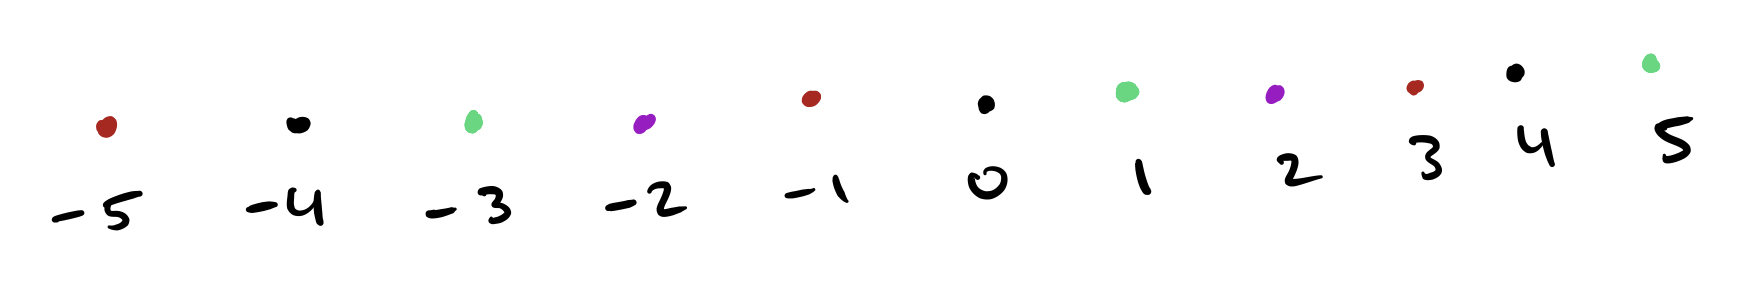
\includegraphics[width=0.75\textwidth]{img/4z}
            \caption{Depicting the cosets of $4 \Z$}
            \label{fig:4z}
        \end{figure}
    }

% hw problem 2 -----------------------------------------------------------------

\newpage
\section*{Alternating group}
    \problem{
        Let $A_5$ stand for all the permutations in $S_5$ that can be written as a composition of an even number of 2-cycles.
        You can take for granted that $A_5$ is a subgroup of $S_5$.
        Find all possible orders of elements of $A_5$.
    }
    \proof{
        First recall that any map $f \in S_5$ can be decomposed into a union of disjoint cycles with length less than or equal to 5.
        Also note that the order of an element $f \in A_5$ is the smallest natural number $m$ to satisfy $f^m = id$.
        We claim that members of $A_5 \leq S_5$ are exactly those maps in $S_5$ which are the union of odd cycle lengths.
        First we show that there exist maps in $A_5$ with odd cycle lengths 1, 2, 3 and 5.
        Since $A_5 \leq S_5$, we know $id \in A_5$ which contains cycles of length 1.
        All of $(12)(23), (12)(34), (12)(23)(34)(45) \in A_5$ for they are a composition of an even number of transpositions.
        To see verification that $(12)(23), (12)(23)(34)(45)$ reduce to cycles lengths of 3 and 5 respectively, see Figure \ref{fig:oddcycle}.
        The map $(12)(34)$ is already simplified as the union of two disjoint 2-cycles.
        \begin{figure}[h]
            \centering
            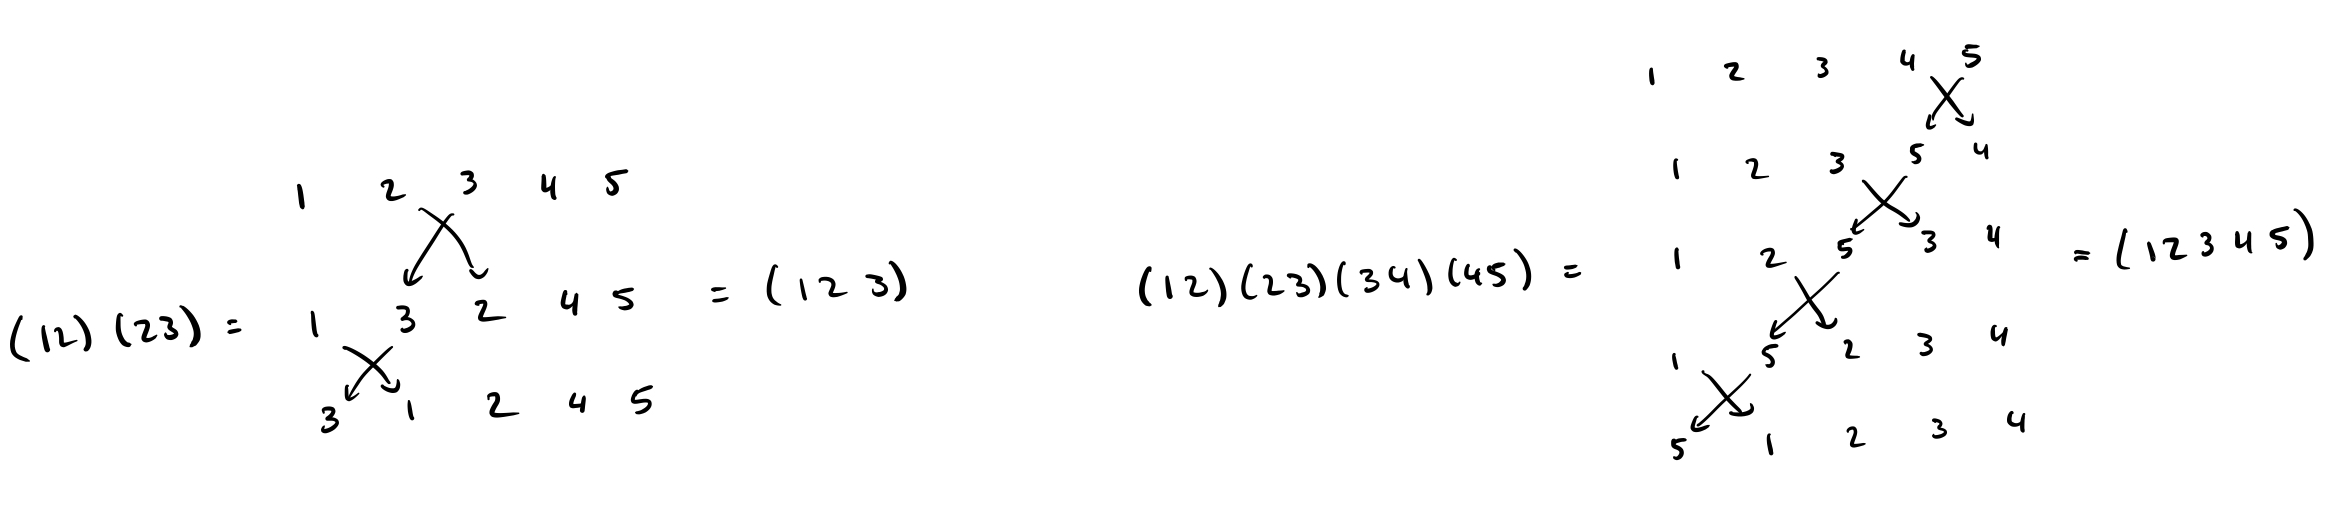
\includegraphics[width=0.95\textwidth]{img/odd-cycle}
            \caption{Showing the existence of odd cycle lengths in $A_5$}
            \label{fig:oddcycle}
        \end{figure} \parspace
        We now argue that now maps with a cycle length of 4 cannot appear in $A_5$.
        Suppose we have a map $f \in S_5$ such that $f$ contains a 4-cycle.
        Then the cycle can be represented as $(a_1 a_2 a_3 a_4) = (a_1 a_2 a_3) (a_3 a_4) = (a_1 a_2) (a_2 a_3) (a_3 a_4)$
        The composition of an odd number of transpotions.
        Indeed, no other decomposition exsts that preserves equality so $f \notin A_4$. \parspace
        Therefore, the possible orders of elements in $A_5$ are 1, 2, 3, 5, and 6.
        We gain 1, 2, 3, and 5 from our examples and 6 by the map which is a composition of a 2 and 3 cycles (evenness will be preserved since even + even is even).
    }


% hw problem 3 -----------------------------------------------------------------

\begin{exercise}{64}{16}
    \problem{
        If $G$ is a finite abelian group and $a_1, a_2, ... , a_n$ are all its elemnts, show that $x = a_1 a_2 \cdots a_n$ must satisfy $x^2 = e$.
    }
    \proof{
        Sorry for the lack of rigor on this problem, I'm rushing to get stuff done today.
        For this problem, we begin with $x = a_1 a_2 \cdots a_n$ and wonder what the value of $x^2 = a_1 a_2 \cdots a_n a_1 a_2 \cdots a_n$ is.
        Since $G$ is abelian, we can rearrange $a_1 a_2 \cdots a_n a_1 a_2 \cdots a_n$ so that each element $a_i$ is next to its inverse $a_i^{-1}$ in $G$.
        By the inverse property of a group we have $x^2 = e^n = e$, which was the goal.
    }
\end{exercise}

% hw problem 4 -----------------------------------------------------------------

\begin{exercise}{64}{15}
    \problem{
        If $p$ is prime, show that the only solutions of $x ^2 \equiv 1 \mod p$ are $x \equiv 1 \mod p$ or $x \equiv -1 \mod p$.
    }
    \proof{
        Consider two cases: $p = 2$ and $p > 2$.
        Let's begin with $p = 2$; we wish to solve $x^2 \equiv 1 \mod 2$.
        Note that $1 \equiv -1 \mod 2$ so we only need to show one equivalence.
        The only options for $x$ are numbers congruent to 0 or 1 mod 2.
        Certainly $0^2 \equiv 0 \mod 2$ is not congruent to 1 mod 2.
        But $1^2 = 1$ is clearly congruent to 1 mod 2. \parspace
        Let's now consider the case where $p > 2$.
        We want to find $x$ such that $x^2 \equiv 1 \mod p \iff p \mid (x^2 - 1) = (x-1)(x+1)$.
        But since $p>2$ we have the equivalent statement that $p \mid (x - 1)$ or $p \mid (x + 1)$.
        This is exactly $x \equiv 1 \mod p$ or $x \equiv -1 \mod p$, so the statement is proved.
    }
\end{exercise}

% hw problem 5 -----------------------------------------------------------------

\begin{exercise}{65}{18}
    \problem{
        Using the results from previous problems, prove that if $p$ is an odd prime number than $(p-1)! \equiv -1 \mod p$.
    }
    \proof{
        Take the finite, abelian group $U _p := \{ k \in \Z _p \mid (k, p) = 1 \} $ with multiplication modulo $p$ (discussed in lecture).
        Since $p$ is prime $U _p = \{ 1, 2, \ldots p-1 \}$.
        By problem 16, the product of every element in $U _p$ squared must be the identity element.
        For our group $U _p$ this means $(p-1)! ^2 \equiv 1 \mod p$.
        But then problem 15 tells us that we must have one of $(p-1)! \equiv 1 \mod p$, $(p-1)! \equiv -1 \mod p$. \parspace
        It remains to be shown that we must have only $(p-1)! \equiv -1 \mod p$ but I struggled to prove this.
        I leave it to be marked off.
    }
\end{exercise}

\end{document}
